
\documentclass[12pt]{article}
\usepackage[usenames,dvipsnames]{color}
\usepackage[utf8]{inputenc}
\usepackage[spanish]{babel}
\usepackage{ragged2e}
\usepackage{graphicx}
\usepackage{amsmath}
\usepackage{cancel}
\usepackage{amsfonts}
\usepackage{amssymb}
\usepackage{anysize}
\usepackage{color}
\usepackage{mathrsfs}
\usepackage{url}
\usepackage{appendix}
\usepackage{amssymb, amsmath, amsbsy}
\usepackage{mathrsfs}
\usepackage{natbib}
\setlength{\parskip}{2ex plus0.7ex minus0.4ex}
\marginsize{3cm}{3cm}{3cm}{3cm}
\fontsize{1000pt}{1000pt} \selectfont 


\title{\color{Black}Detección de Alzheimer en Imágenes de Resonancia Magnética
 por Medio de Morfología Matemática y Computación.}
\author{Universidad Nacional de Colombia - Matemáticas Discretas II \\  Grupo: Mano invisible \\
\\
Prof. Andrés Villaveces Niño} 
\date{Diciembre 05, 2015}
\pagestyle{plain}
\begin{document}
\raggedright{}
\maketitle{Miguel Ángel Ballén Galindo \hspace{5.72cm} \ \ Código: 2879490 \\}
\maketitle{Carlos Arturo López Romero \hspace{5.99cm} Código: 2274441\\}
\maketitle{Cristian Andres Garcia Prieto\hspace{5.7cm} \ \ Código: 2879608\\}


\rule{150mm}{0.5mm}
\maketitle
\newpage
\tableofcontents
\newpage


\section{\color{Black}Planteamiento del problema}
\justifying

Dentro de los trastornos cerebrales conocidos, se halla que uno de los trastornos más estudiados es el Alzheimer. Esta enfermedad se caracteriza porla perdida de las funciones intelectuales superiores, con alteraciones del ánimo y la conducta y también se sabe que es la causa mas común de demencia en el anciano.

Luego de haber avanzado el trastorno, se presenta una desorientación y perdida de la memoria y conforme avanza la enfermedad se evidencia una Afasia progresiva... Indicando una disfunción Cortical grave. 
Finalmente con el paso del tiempo ( entre 5 a 15 años) el paciente aparecerá profundamente discapacitado, con mutismo e inmóvil. Rara vez se presenta antes de los 50 años, pero la incidencia aumenta cada 5 años aproximadamente. Es decir que la incidencia en la población de 60 a 64 años es de 1\% y en la población de 85 a 89 años se eleva para un 40\%; lo cual crea una necesidad de diagnóstico temprano y prevención de la enfermedad\cite[pag 1325]{kumar2010robbins}.

A medida que la ciencia avanza se han utilizado diferentes métodos para la detección temprana de dicha de dicha enfermedad, entre las que se encuentran la tomografía por emisión de positrones (PET), la tomografía por emisión de  foto único (SPECT), la resonancia magnética funcional (fMRI) y las imágenes de resonancia magnética (RMN) \cite{masdeujose2004}, sin embargo, se cree que esta última pueden no ser muy precisa debido a la dificultad de observar anomalías cerebrales en las fases tempranas de la enfermedad.




\begin{figure}[htb]
\centering
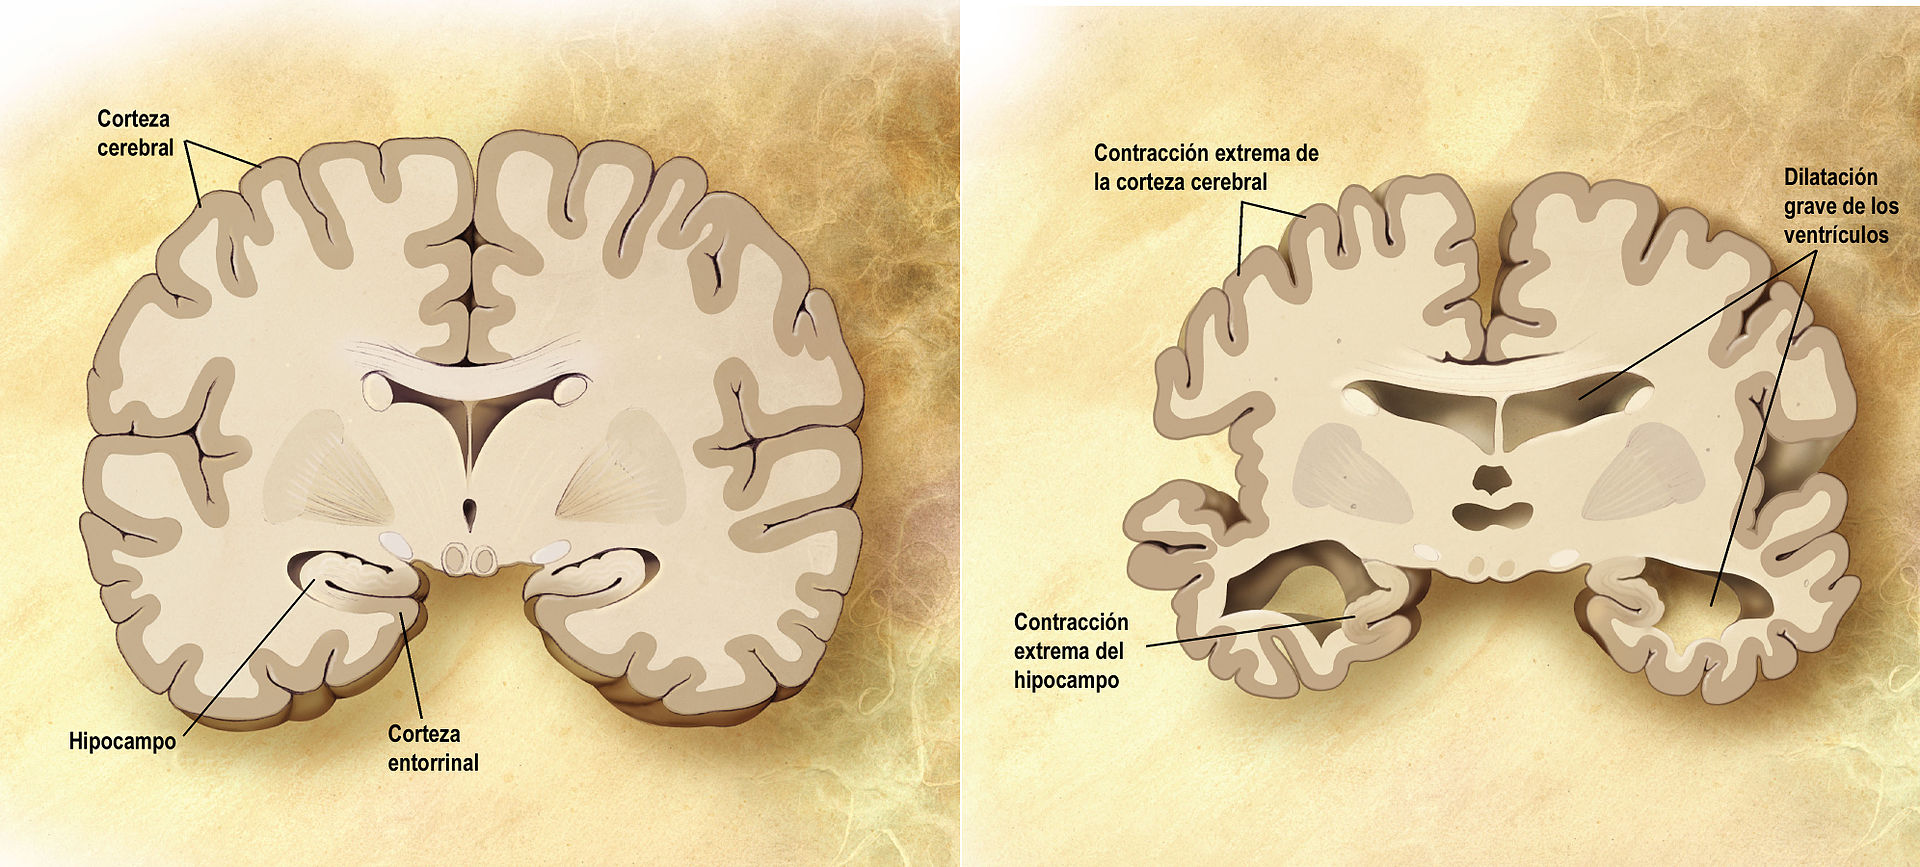
\includegraphics[width=0.95\textwidth]{Alzheimer}
\caption{Comparación entre un cerebro normal y un cerebro afectado de alzheimer\cite{wiki:Alz}} \label{A1}
\end{figure}

 Las nuevas tecnologías de procesamiento de imagen permiten el tratamiento computacional de las imágenes obtenidas a través RMN, por lo tanto, por medio de algoritmos es plausible la detección de patrones asociados a cambios estructurales del tejido cerebral característicos del el Alzheimer, aumentando la probabilidad de detectar la enfermedad en una fase temprana. 
 
 Por lo anterior el proyecto expuesto en el presente documento,  se enfoca en determinar la probabilidad de presencia de Alzheimer a través de la creación de un modelo computacional. Como es posible ver  en la figura \ref{A1} existe una clara disminución de la masa cerebral del paciente, lo cual conlleva a una contracción de las capas externas de la Corteza Cerebral, a una dilatación grave de los Ventrículos y a una contracion del Hipocampo. 

  
\section{\color{Black}Marco Teórico}
\justifying

Una imagen digital, es una función que se ha discretizado tanto en coordenadas espaciales, como en nivel de brillo siendo esta la función aplicada. Cada uno de los pixeles de una imagen representa un elemento de este conjunto, dentro del cual se realizan las diferentes operaciones.

Según el modelo propuesto por \cite{benalcazar2014aprendizaje}, una imagen puede representarse computacionalmente como una matriz de M x N, cuyas entradas corresponden al nivel de gris de un pixel (Figura \ref{f1}). Siendo E un subconjunto  finito y no vacío de $Z^2$, y $L = (l_{min},...,l_{max})$ con $l=$ $ \mid L \mid $ el conjunto de niveles de gris de una imagen.Por tanto, una imagen digital en escala de grises es una función $O: E \rightarrow L$, cuyo tamaño es el número de píxeles de la misma, siendo un pixel $t(x,y)$ una de las entradas de la matriz. El conjunto de todas las imágenes con dominio E y rango L se denomina con $L^E$.

Una imagen Binaria, consiste en una matriz cuyas entradas vienen determinadas por una función $O: E \rightarrow \{0,1\}$ que corresponde a un caso particular de la definición de O; cuando el conjunto de niveles de escala de gris es $L = \{0,1 \} $.

\begin{figure}[htb]
\centering
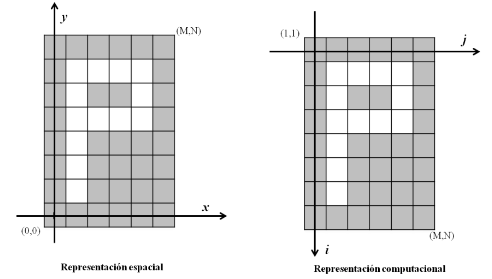
\includegraphics[width=0.7\textwidth]{g1}
\caption{Representación espacial y computacional de una imagen \cite{benalcazar2014aprendizaje}} \label{f1}
\end{figure}


\subsection{\color{Black}Operaciones Morfológicas Fundamentales}
\justifying

De acuerdo con las diferentes fuentes empleadas, se sabe que para realizar el procesamiento de imágenes es necesario aplicar una conjunto básico de Operaciones Morfológicas Fundamentales, consistentes en la modificación de los elementos de un conjunto, o imagen como se detallará más adelante.

Es importante mencionar que muchas de estas operaciones son utilizadas de manera combinada en los algoritmos definidos para el tratamiento. Pues de esta forma se facilita la comprensión de la metodología empleada en este proyecto. 

Las operaciones fundamentales funcionan de acuerdo con un \textbf{\textit {Elemento Estructurante o Kern...}}

\justifying
Se define el conjunto:

\centering
$B=\{b_{1},...,(0,0),...,b_{n}\}$
 \newline como \textit{Kern} de una imagen. 

\justifying
En todos los procesos de tratamiento de imágenes, se establece una forma determinada para el \textit{ Kern B} y el tamaño que entraría a cambiar el conjunto de la imagen, de acuerdo con el resultado final buscado.

A continuación se definen las 4 operaciones fundamentales de Morfología Matemática, basados en \cite{villaveces}.

\textbf{\textit{Suma De Minkowski:}}
\begin{equation}
\centering
\textbf{$X \oplus Y := \{ x+y \mid x \in X, y \in Y \}$   }
\end{equation}

\justifying
\textbf{\textit{Dilatación Binaria:}}

La Dilatación Binaria para un conjunto X por medio de \textit{Elemento Estructurante}. Expresando la suma de Minkowski, de X con el simétrico de B con respecto a su centro $(\check{B})$:

\begin{equation}
\centering
\textbf{
$ D(X,B) :=  X \oplus \check{B} = \{x+y \mid x \in X, y \in \check{B} \}$ 
}
\end{equation}
              
\justifying Operación bajo la cual se logra el adelgazamiento de los objetos que componen la imagen de acuerdo con el $kern$ empleado, obteniendo la intersección no vacía con el conjunto o imagen inicial X.   
              
\textbf{\textit{Erosión Binaria:}} 

La Erosión de un conjunto X por un Elemento Estructurante B, se encuentra definida como: 

\begin{equation}
E(X,B) := x \ominus \check{B} = \{ x \mid \forall y \in B, x+y \in X  \}
\end{equation}

También definida, como:

\begin{equation}
                E(X,B) := \{ x \in \mathbb{R^n} \mid B_{x} \subset X \}
\end{equation}


\justifying
   Operación bajo la cual se logra el engrosamiento de los bordes de los objetos que componen la imagen con el $kern$ empleado, es decir $\check{B}$, obteniendo contenencia dentro del conjunto o imagen inicial X.
   
\justifying   
\textbf{\textit{Apertura Binaria:}} La $Apertura Binaria$ de un conjunto o imagen X, por medio del elemento estructurante B, viene determinada por una composición de los operadores de Dilatación y Erosión Binarias, como se define a continuación:


\begin{equation}
X_{B} := D[E(X,B),\check{B}]
\end{equation}

\justifying
\textbf{\textit{Cerradura Binaria:}} 

La $Cerradura Binaria$ de un conjunto o imagen X, por medio del elemento estructurante B, viene determinada por una composición de los operadores de Dilatación y Erosión Binarias, como se define a continuación:

\begin{equation}
X^B := E[D(X,B), \check{B}]
\end{equation}

 \justifying
 Con los conceptos Fundamentales Morfológicos claros, es admisible presentar los algoritmos empleados para el análisis de las imágenes diagnósticas, como se desarrollan a continuación.
   
                
\
\justifying
\subsection{\color{Black}Transformacion de Top-Hat}
\justifying

Normalmente después de aplicar erosión o dilatación en una imagen es muy difícil obtener nuevamente la imagen original, sin embargo, involucrando estas operaciones básicas en conjunto podríamos obtener una imagen parecida a la original, bien sea por dilatación de la imagen resultante de una erosión, o por el contrario erosionar la imagen resultante de una dilatación, dichas operaciones se conocen como apertura $\gamma(f)$  y cierre $\varphi(f)$ respectivamente. El problema es que el resultado de ejecutarlas solo aproxima la imagen original haciendo que se pierda o se agreguen conexiones en la imagen, de tal manera que para solucionar este problema se emplea la transformación de Top-Hat, la cual permite con un kern adecuado encontrar las conexiones en la imagen que se habían perdido al efectuar las operaciones, tal como se  puede observar en la figura \ref{f2}.


\begin{figure}[htb]
\centering
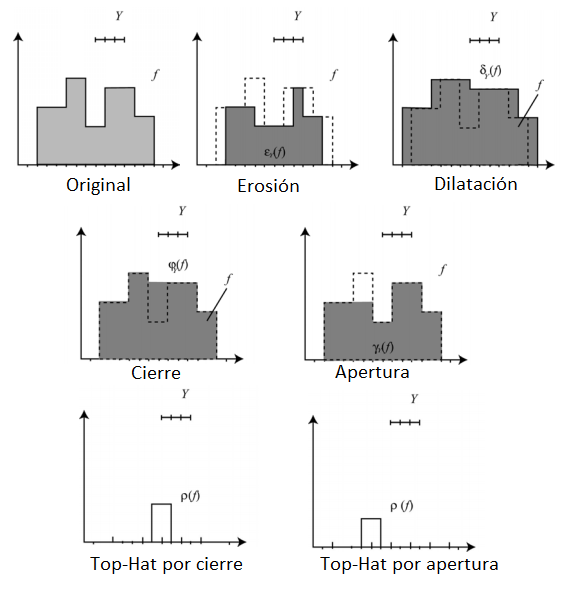
\includegraphics[width=0.44\textwidth]{imagen2}\\
\caption{ Operaciones morfológicas fundamentales aplicadas para un Kern unidimensional mas Top-Hat de Apertura y de Cierre para el mismo \cite{ortiz2002procesamiento} } \small
\label{f2}
\end{figure}

Si quiere hacer un Top- Hat por apertura, simplemente se toma la imagen original y se le resta la apertura de la imagen, esto devuelve la estructura de la imagen que se pierde al aplicar una apertura. Por otro lado, si se aplica Top-Hat por cierre, en el cual se toma el cierre y se resta la imagen original se obtiene la estructura de la imagen que se agregó al aplicar el cierre \cite{ortiz2002procesamiento}. Matemáticamente se puede definir como dos operaciones duales, siendo f una imagen arbitraria:

\begin{equation}
\rho(f) = f - \gamma(f)
\end{equation}

\begin{equation}
\rho(f) = \varphi(f) - f
\end{equation}

\subsection{\color{Black}Método de Otsu}
\justifying

La binarización de imágenes es un paso crucial en la segmentación de imágenes, pero no se trata de un proceso arbitrario, ya que definir un umbral será lo que permite  separar el fondo de la escena de las estructuras. El umbral puede depender de la imagen a escala de grises \textit{f(x,y)} , de una propiedad local de la ubicación (valor promedio d los pixeles cercanos ) o de la ubicación. Pese a la existencia de diversos métodos para hallar umbrales, la existencia de ruido, histogramas planos, etc. hace que la mayoría de estos no sean recomendables.
Una imagen digital, es una función que se ha discretizado tanto en coordenadas espaciales, como en nivel de brillo siendo esta la función aplicada.Tomando la definición de \cite{Otsu} cada uno de los pixeles de una imagen representa un elemento de este conjunto entre \textit{1} y \textit{L}, dentro del cual se realizan las diferentes operaciones. El numero de pixeles con nivel \textit{i} de gris se denota $f_{i}$ y la probabilidad de este \textit{i} esta dada por:

\begin{equation}\label{ec1}
p_{i} = \frac{f_{i}}{N}
\end{equation}

En el caso de la binarizacion los pixeles son divididos en 2 clases, $C_{1}$ con niveles de gris $[1, ..., t]$; y $C_{2}$ con niveles de gris $[t+1, ..., L]$, y la distribución de las probabilidades son:

\begin{equation}
C_{1} : \frac{P_{1}}{\omega_{1}(t)}, ..., \frac{P_{t}}{\omega_{1}(t)}
\end{equation}

\begin{equation}
C_{2} : \frac{P_{t+1}}{\omega_{2}(t)}, \frac{P_{t+2}}{\omega_{2}(t)} ..., \frac{P_{L}}{\omega_{2}(t)}
\end{equation}

donde

\begin{equation}
\omega_{1}(t) = \sum_{i=1}^t P_{i} \qquad \omega_{2}(t) = \sum_{i=t+1}^L P_{i}
\end{equation}

La media para $C_{1}$ y $C_{2}$ es:

\begin{equation}
\mu_{1} = \sum_{i=1}^t \frac{i.P_{i}}{\omega_{1}(t)} \qquad \mu_{2} = \sum_{i=t+1}^L \frac{i.P_{i}}{\omega_{2}(t)}
\end{equation}

y sea $\mu_{T}$ la intensidad media de toda la imagen.Entonces

\begin{equation}
\omega_{1}.\mu_{1}+\omega_2.\mu_{2}=\mu_{T} \qquad \omega_{1}+\omega_{2}=1
\end{equation}

Y así Otsu definió la varianza entre clases de una imagen como:

\begin{equation}\label{var}
\sigma_{B}^2=\omega_{1}.(\mu_{1}-\mu_{T})^2+\omega_{2}.(\mu_{2}-\mu_{T})^2
\end{equation}

Otsu verifico que el umbral optimo $t^*$ selige de manera que la ecuación  \ref{var} sea máxima esto en la binarizacion de 2 niveles:

\begin{equation}
t^*= \max{\{\sigma_{B}^2(t)\}} \qquad \qquad 1\leq t \leq L
\end{equation}
De este modo podemos calcular un umbral optimo para que al binarizar la imagen no perdamos los pequeños limites que son necesarios para llevar a cabo nuestro objetivo

\subsection{\color{Black}Segmentación Watershed (Línea divisora de Aguas)}
\justifying

La segmentación WaterShed es un algoritmo comúnmente empleado para encontrar regiones de una imagen con texturas homogéneas y es ampliamente utilizado para el análisis de imágenes médicas. Dentro de sus funciones, permite extraer las fronteras de las regiones existentes en una imagen; clasificando los pixeles según su proximidad espacial, el gradiente de sus niveles de gris, y la homogeneidad de sus texturas. El algoritmo WaterShed popuesto por Vincent y Soille (1991), ordena los pixeles según su nivel de gris en una estructura de datos tipo pila, para empezar el proceso de inundación de las vasijas o puntos mínimos de la imagen.Según \cite{palomino2010watershed} durante el proceso de inundación, se producen hasta tres casos posibles:

\begin{enumerate}
	\item Crecimiento de un basin ya existente en \textit{Zi(f)}. En este 
caso, si el valor del pixel de las imágenes que se com
paran, es decir \textit{Zi+1(f)} es mayor que \textit{Zi(f)}, se produce 
el crecimiento (inundación) del basin \textit{Wi(f)}, es decir se 
genera \textit{Wi+1(f)}, si son iguales el basin permanece con 
igual tamaño.
	\item Aparición de una nueva basin, si el valor del pixel de las 
imágenes que se comparan, es decir \textit{Zi+1(f)} es menor 
que \textit{Zi(f)}, aparecen nuevas regiones de inundación, es 
decir, nuevas basin.
	\item Determinación de zonas de influencia, si la inundación 
del nivel \textit{i+1} une basins inundadas del nivel \textit{i}, se deben 
separar las regiones utilizando las zonas de influencia 
de cada componente conectada. En este caso, la basin de \textit{i+1}, es decir \textit{Wi+1} son zonas de influencia de la 
basin \textit{Wi}.
\end{enumerate}
\begin{figure}[htb]
\centering
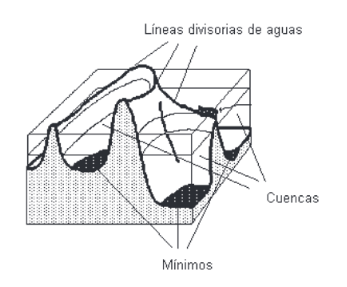
\includegraphics[width=0.42\textwidth]{water}\\
\caption{ Líneas divisorias, cuencas y mínimos \cite{palomino2010watershed} } \small
\label{f3}
\end{figure}




\section{\color{Black}Objetivo}
\justifying

Crear un modelo computacional, que permita detectar algunos de los patrones presentes en imágenes de Resonancia Magnética, que permitan concluir con cierto grado de certeza, la posible pérdida de células cerebrales, determinando una probabilidad de presencia del trastorno de Alzheimer

\section{\color{Black}Metodología}
\justifying
Se obtuvo acceso a la base de datos de imágenes diagnósticas del proyecto Alzheimer Disease Neuroimaging initiative (ADNI) de la Universidad Del Sur De California(figura \ref{bd}) \cite{BaseDatos} de la cual se extrajeron imágenes diagnósticas con el objetivo de aplicar un modelo computacional con ayuda del programa Matlab versión R2015b

\begin{figure}[htb]
\centering
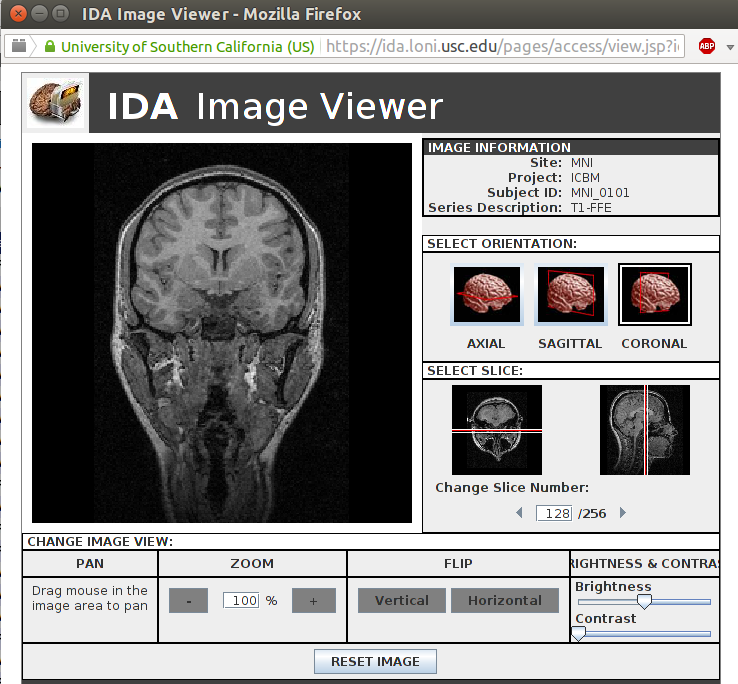
\includegraphics[width=0.44\textwidth]{patient}\\
\caption{Imágenes diagnosticas de la plataforma Alzheimer Disease Neuroimaging initiative (ADNI) de la Universidad Del Sur De California.\cite{BaseDatos} } \small
\label{bd}
\end{figure}

Como procedimiento inicial , las imágenes originales fueron convertidas en imágenes a escala de grises para poder realizar las operaciones fundamentales.

Para cada imagen se determinó el elemento estructurante \textit{B} y se aplica la  reflexión  del mismo $\check{B}$ y traslación $B_{t}$. Posteriormente, se aplicó erosión y dilatación. Con el fin de obtener las partes más claras de las imágenes se aplicó el método de Top-Hat por apertura.

Previo al proceso de segmentación se aplicó el método de Otsu, el cual consiste en binarizar la imagen hallando el umbral óptimo para cada imagen y hacerlo de la manera menos arbitraria posible.

Una vez binarizada la imagen, se aplicó la segmentación WaterShed siguendo la metodología propuesta por Palomino \& Concepción (2010) \cite{palomino2010watershed}.).  En la cual a cada uno de los mínimos de la imagen se le asigna una etiqueta diferente que se propaga a todos los pixeles adyacentes en un nivel dado. En cada paso se analizaron los componentes conectados entre la vitalización en \textit{h} y \textit{h+1}. Al final de la inundación todos los pixeles menos las líneas Watershed tenían una etiqueta que indicadora de la región a la cual pertenecían. El negativo de las regiones inundadas, forman las líneas Watershed que separan las distintas regiones de la imagen que crecieron a partir de los mínimos regionales. El proceso de inundación en las vasijas o basin se realizó comparando la imagen \textit{f}, binarizada con un umbral \textit{i}, que se denota \textit{Zi(f)}, y la imagen en un nivel superior \textit{Zi+1(f)}, desde $i = 0$ hasta $i = N$, donde \textit{N} es el máximo nivel de gris con que se representa la imagen. En cada nivel \textit{i} de la imagen \textit{f} se tienen mínimos regionales \textit{mi(f)}. La vasija o basin de la imagen f en el nivel de \textit{i}, se denota \textit{Wi(f)}, que inicialmente son los mínimos regionales.
\textit{Wi+1(f)} es el resultado de la inundación de la basin \textit{Wi(f)}.

\section{\color{Black}Resultados y Discusión}
\justifying

 %%Pendiente Descripción de los resultados%%
 
 
 
 \begin{figure}[htb]
\centering
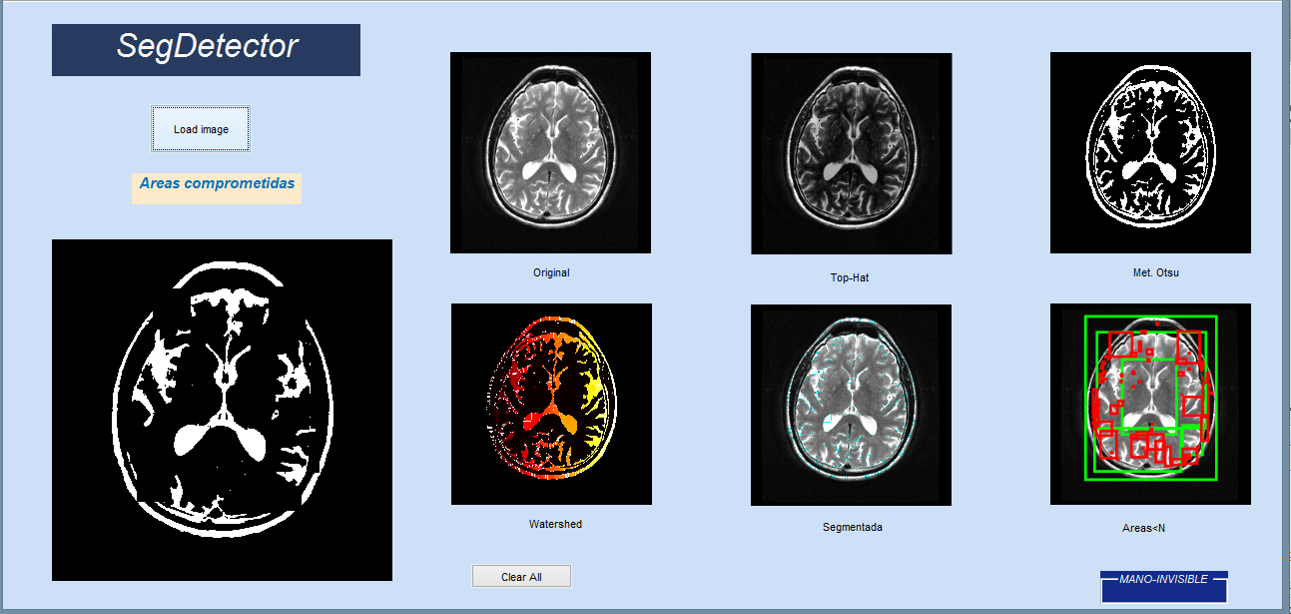
\includegraphics[width=0.77\textwidth]{Resultado}\\
\caption{ Imagen resultante de aplicar el programa a una paciente con Alzheimer } \small
\label{rs}
\end{figure}
 
Cabe aclarar que las anomalías aunque pueden ser patológicas degenerativas, el código está orientado a resolver el problema específico del diagnóstico temprano de enfermedad de Alzheimer, detectando cambios en la corteza cerebral como la contracción y engrosamiento de dicha estructura, también es capaz de identificar la dilatación de ventrículos en un corte $Axial$.

Se observa que al cargar una imagen de un paciente control el resultado de esta será una imagen que cubre el total del área del cerebro ya que no presenta una anomalía. Adicionalmente, podemos ver que la elección del Kern se realizó como ensayo y error; pero  se debe tener presente que las formas que buscamos están directamente relacionadas con un disk (disco) ya que cubre todas las áreas en la misma dirección y el tamaño está directamente relacionado con el tamaño de la corteza cerebral

\section{\color{Black}Conclusiones}

Es posible concluir que el código escrito para este documento  tiene un resultado satisfactorio para identificar anomalías fisiológicas o cambios estructurales en el cerebro y por tanto podría ser considerado como una herramienta de diagnóstico médico en un futuro.

Gracias a la velocidad consgrada en muchas de las máquinas construidas actualmente; es válido afirmar que el acoplamiento de la Teoría de Conjuntos con los algoritmos empleados en las distintas aplicaciones de Morfología Matemática, nos presentan una herramienta combinada de gran utilidad.

Esta afirmación se explica gracias a muchos de los estudios similares al tratado en este proyecto. Por lo que es comprensible que se establezcan nuevos métodos para tratamiento de imágenes y nuevas formas de detección, prevención y tratamiento de enfermedades... Que con certeza, antes eran más difíciles de comprobar.




\newpage
\section{\color{Black}Bibliográfia}
\bibliographystyle{alpha}
\bibliography{Biblio}

\end{document}

